\documentclass{article}
\usepackage{indentfirst}
\usepackage[utf8]{inputenc}
\usepackage[T1]{fontenc}
\usepackage[brazilian]{babel}
\usepackage{lmodern}
\usepackage{graphicx}
\usepackage{float}
\usepackage[]{subfigure}
\usepackage{afterpage}
\usepackage{amsmath}
\usepackage{textcomp,gensymb}
\usepackage{nameref}
\usepackage{accents}
\usepackage{listings}
\usepackage{color,soul}
\usepackage[margin=1in]{geometry}
\usepackage{steinmetz}

\PassOptionsToPackage{hyphens}{url}\usepackage{hyperref}
\hypersetup{
    breaklinks = true,
}
\urlstyle{same}
\newcommand{\ubar}[1]{\underaccent{\bar}{#1}}
\renewcommand\thesection{\arabic{section}$^a$}
\renewcommand\thesubsection{(\alph{subsection})}
\definecolor{dkgreen}{rgb}{0,0.6,0}
\definecolor{gray}{rgb}{0.5,0.5,0.5}
\definecolor{mauve}{rgb}{0.58,0,0.82}
\lstset{
    frame=tb,
    language=Matlab,
    aboveskip=3mm,
    belowskip=3mm,
    showstringspaces=false,
    basicstyle={\small\ttfamily},
    numbers=none,
    numberstyle=\tiny\color{gray},
    keywordstyle=\color{blue},
    commentstyle=\color{dkgreen},
    stringstyle=\color{mauve},
    breaklines=true,
    breakatwhitespace=true,
    tabsize=4
}

\title{Trabalho}
\author{Arthur Matos}
\date{2019}

\begin{document}
% capa
\begin{titlepage}
    \begin{center}
        \centering
        
\includegraphics[width=.7\linewidth]{images/LogoUnB.png}\\[0.5cm]
        {\large \textbf{Universidade de Brasília}}\\[0.2cm]
        {\large \textbf{Departamento de Engenharia Elétrica}}\\[0.2cm]
        {\large \textbf{Controle Digital}}\\[4.8cm]
        {\bf \huge {Exercício de Simulação 5}}\\[0.2cm]
        {\bf \large {}}
    \end{center}

    \vspace{5cm}
    \hspace{2cm} {\noindent \bf \large {Aluno:}}\\
    \vspace{0.8cm}
    \hspace{2.35cm} {\large Arthur de Matos Beggs --------------------------------- 12/0111098}\\[1cm]

    \begin{center}
        {\large Brasília}\\
        {\large 1$^{\ubar{\circ}}$/2020}
    \end{center}

\end{titlepage}
\clearpage
\setcounter{page}{2}
% \tableofcontents
\clearpage

% % Template de figura
% \begin{figure}[H]
%     \centering
%         \includegraphics[width=1\linewidth]{images/}
%         \caption{}\label{fig:}
% \end{figure}

% % Corpo do Relatório

\section*{Questão 1}
    {Para um processo descrito pela função de transferência}

    $$ G(z) = \frac{ 0.0125(z+0.195)(z+2.821) } { z(z-1)(z-0.368)(z-0.8187) } $$

    {\textbf{a)}}

    $$ G(z) = \frac{ 0.0125(z+0.195)(z+2.821) } { z(z-1)(z-0.368)(z-0.8187) } = \frac{ 0.0125z^{-2}(1+0.195z^{-1})(1+2.821z^{-1}) } { (1-z^{-1})(1-0.368z^{-1})(1-0.8187z^{-1}) } $$

    $$ p = max\{ 1,1 \} = 1 $$
    $$ n = 4-2 = 2 \implies k \geq n = 2 $$\\[0.1cm]

    {Para tempo mínimo, $ k=2 $}\\[0.1cm]

    $$ M(z) = (1+2.821z^{-1})(?)_1 $$
    $$ (?)_1 = (M_2 z^{-2} + \dots) \implies M(z) = (1+2.821z^{-1})(M_2 z^{-2} + \dots) $$


    $$ 1-M(z) = (1-z^{-1})(?)_z $$
    $$ (?)_z = (1+ a_1 z^{-1} + \dots) \implies 1-M(z) = (1-z^{-1})(1+ a_1 z^{-1} + \dots) $$

    $$ 1- (1+2.821z^{-1})(M_2 z^{-2} + \dots) = (1-z^{-1})(1+ a_1 z^{-1} + \dots) $$\\[0.1cm]

    {Para manter o maior grau da equação como 3 ($z^{-3}$),}

    $$ 1- (1+2.821z^{-1})M_2 z^{-2} = (1-z^{-1})(1+ a_1 z^{-1} + a_2 z^{-2}) $$

    $$ M(z) = (1+2.821z^{-1})M_2 z^{-2} $$
    $$ 1-M(z) = (1-z^{-1})(1+ a_1 z^{-1} + a_2 z^{-2}) $$

    $$ 1 - M_2 z^{-2} - 2.821M_2 z^{-3} = 1 + a_1 z^{-1} + a_2 z^{-2} - z^{-1} - a_1 z^{-2} - a_2 z^{-3} $$
    $$ 1 - M_2 z^{-2} - 2.821M_2 z^{-3} = 1 + (a_1 -1)z^{-1} + (a_2 - a_1)z^{-2} - a_2 z^{-3} $$

    \[
        \begin{cases}
            a_1 - 1 = 0\\
            M_2 = a_1 - a_2\\
            2.821M_2 = a_2\\
        \end{cases}
        \implies
        \begin{cases}
            a_1 = 1\\
            a_2 = 0.7383\\
            M_2 = 0.2617\\
        \end{cases}
    \]\\

    \clearpage

    $$ M(z) = (1 + 2.821z^{-1})0.2617z^{-2} = \frac{ 0.2617(z+2.821) }{ z^3 } $$

    $$ 1-M(z) = (1-z^{-1})(1 + z^{-1} + 0.7383z^{-2}) = \frac{ (z-1)(z^2 + z + 0.7383) }{ z^3 } $$

    $$ G_{D}(z) = \frac{1}{G(z)} \frac{M(z)}{1-M(z)} = \frac{ z(z-1)(z-0.368)(z-0.8187) }{ 0.0125(z+0.195)(z+2.821) } \frac{ \frac{0.2617(z+2.821)} {z^3} }{ \frac{ (z-1)(z^2 + z + 0.7383) }{ z^3 } } $$\\[0.1cm]

    $$ G_{D}(z) = \frac{ 20,936z(z-0.368)(z-0.8187) }{ (z+0.195)(z^2 + z + 0.7833) } $$\\[0.5cm]

    {\textbf{b)}}

    \begin{figure}[H]
       \centering
            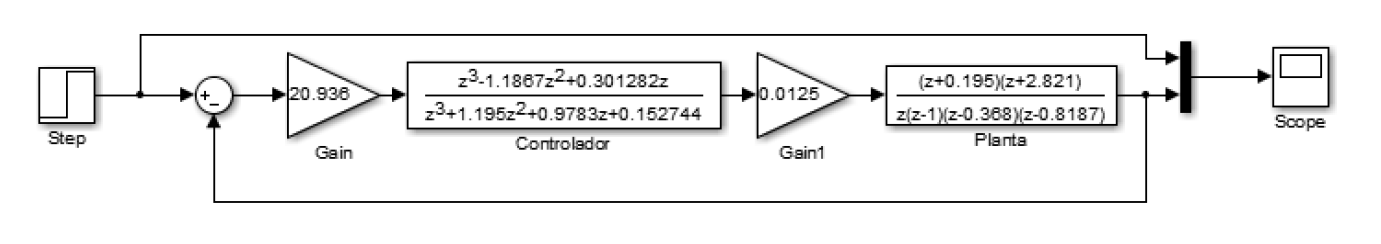
\includegraphics[width=1\linewidth]{images/diagrama1b.png}
            \caption{Diagrama do sistema.}
            \label{fig:diagram1b}
    \end{figure}

    \begin{figure}[H]
       \centering
            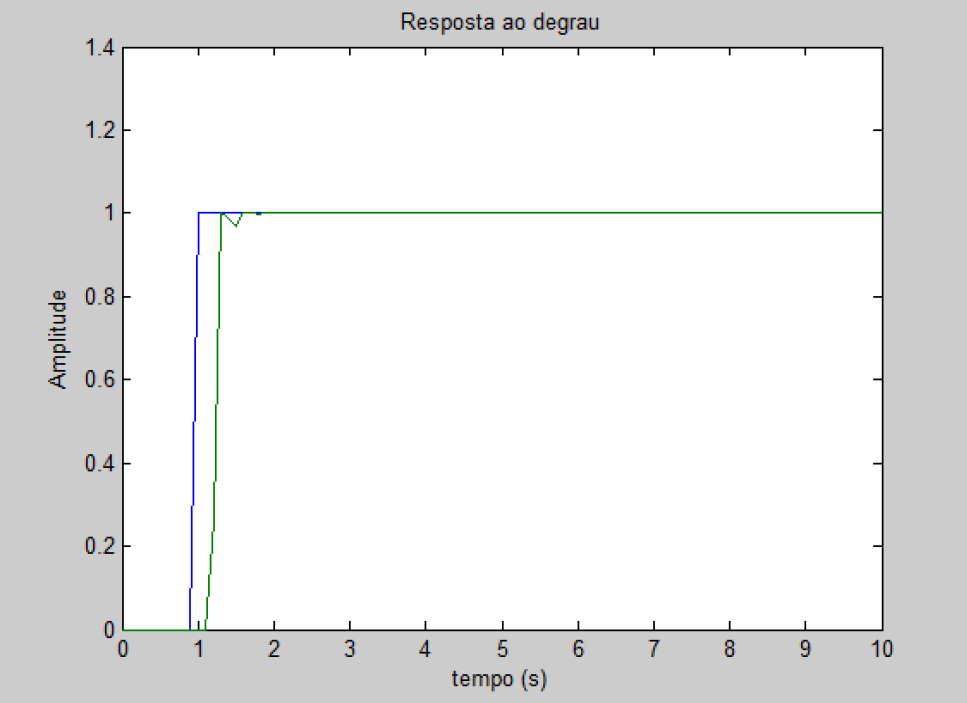
\includegraphics[width=.7\linewidth]{images/grafico1b.png}
            \caption{Resposta ao degrau.}
            \label{fig:graph1b}
    \end{figure}

    \clearpage

    {\textbf{c)}}

    $$ p = max\{ 2,1 \} = 2 $$
    $$ n = 4-2 = 2 \implies k \geq n = 2 $$\\[0.1cm]

    $$ 1- (1+2.821z^{-1})(M_1 z^{-1} + M_2 z^{-2}) = (1-z^{-1})^2 (1+ a_1 z^{-1}) $$

    $$ M(z) = (1+2.821z^{-1})(M_1 z^{-1} + M_2 z^{-2}) $$
    $$ 1-M(z) = (1-z^{-1})^2 (1+ a_1 z^{-1}) $$


    $$ 1 - M_1 z^{-1}  - M_2 z^{-2} - 2.821M_1 z^{-2} - 2.821M_2 z^{-3} = 1 + a_1 z^{-1} - 2z^{-1} -2a_1 z^{-2} + z^{-2} +a_1 z^{-3} $$


    $$ 1 - M_1 z^{-1} - (M2 + 2.821M_1) z^{-2} - 2.821M_2 z^{-3} = 1 + (a_1 - 2)z^{-1} + (1 - 2a_1)z^{-2} + a_1 z^{-3} $$

    \[
        \begin{cases}
            a_1 - 2 = -M_1\\
            1 - 2a_1 = -M_2 - 2.821M_1\\
            a_1 = 2.821M_2\\
        \end{cases}
        \implies
        \begin{cases}
            a_1 = 1.2833\\
            M_1 = 0.7167\\
            M_2 = -0.46493\\
        \end{cases}
    \]\\

    $$ M(z) = (1+2.821z^{-1})(0.7167z^{-1} - 0.46493z^{-2}) = \frac{ 0.7167(z+2.821)(z-0.63475) }{ z^3 } $$

    $$ 1-M(z) = (1-z^{-1})^2 (1+ 1.2833 z^{-1}) = \frac{ (z-1)^2 (z + 1.2833) }{ z^3 } $$

    $$ G_{D}(z) = \frac{1}{G(z)} \frac{M(z)}{1-M(z)} = \frac{ z(z-1)(z-0.368)(z-0.8187) }{ 0.0125(z+0.195)(z+2.821) } \frac{ \frac{ 0.7167(z+2.821)(z-0.63475) }{ z^3 } }{ \frac{ (z-1)^2 (z + 1.2833) }{ z^3 } } $$\\[0.1cm]

    $$ G_{D}(z) = \frac{ 57.336z(z-0.368)(z-0.8187)(z-0.63475) }{ (z-1)(z+0.195)(z+1.2833) } $$\\[0.5cm]


    {\textbf{d)}}

    \begin{figure}[H]
       \centering
            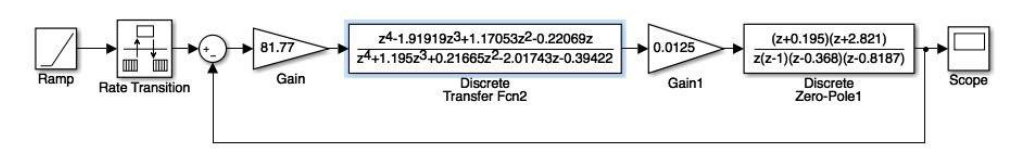
\includegraphics[width=1\linewidth]{images/diagrama1d.png}
            \caption{Diagrama do sistema.}
            \label{fig:diagram1d}
    \end{figure}

    \begin{figure}[H]
       \centering
            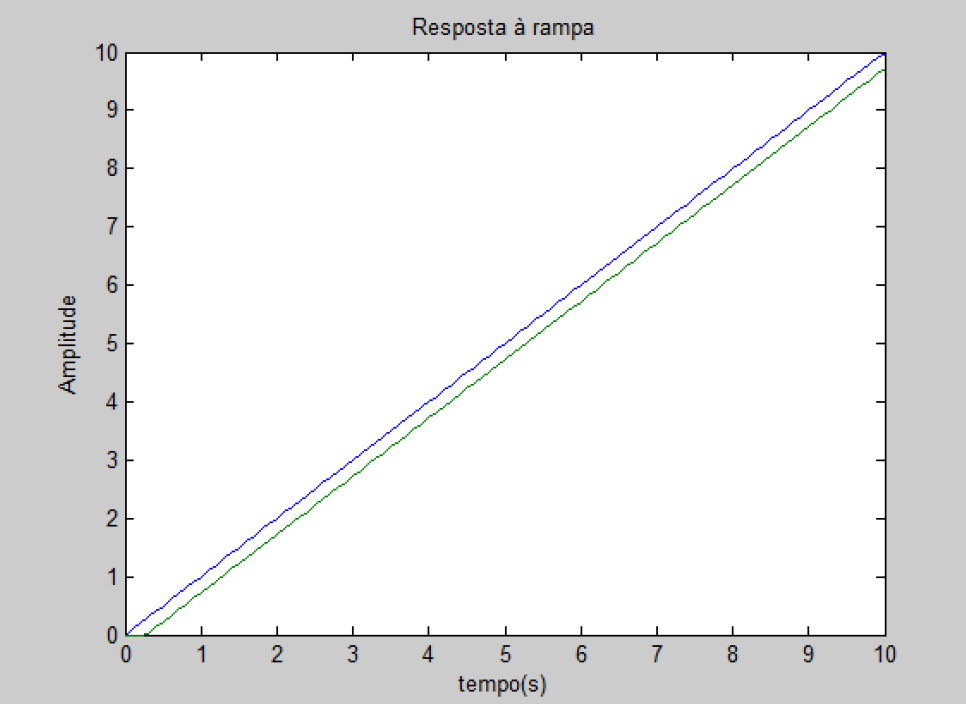
\includegraphics[width=.7\linewidth]{images/grafico1d.png}
            \caption{Resposta à rampa.}
            \label{fig:graph1d}
    \end{figure}

    \vspace{5mm}


\section*{Questão 2}
    {Para um processo descrito pela função de transferência}

    $$ G(z) = \frac{ 0.0003916(z+2.8276)(z+0.19) }{ (z-1)^2 (z-0.2865) } $$

    {\textbf{a)}}

    $$ p = max\{ 2,1 \} = 2 $$
    $$ n = 3-2 = 1 \implies k \geq n = 1 $$\\[0.1cm]

    $$ M(z) = (1+2.8276z^{-1})(M_1 z^{-1} + \dots) $$

    $$ 1-M(z) = (1-z^{-1})^2 (1+ a_1 z^{-1} + \dots) $$

    $$ 1- (1+2.8276z^{-1})(M_1 z^{-1} + \dots) = (1-z^{-1})^2 (1+ a_1 z^{-1} + \dots) $$\\[0.1cm]

    {Para manter o maior grau da equação como 3 ($z^{-3}$),}

    $$ 1- (1+2.8276z^{-1})(M_1 z^{-1} + M_2 z^{-2}) = (1-z^{-1})^2 (1+ a_1 z^{-1}) $$

    $$ M(z) = (1+2.8276z^{-1})(M_1 z^{-1} + M_2 z^{-2}) $$
    $$ 1-M(z) = (1-z^{-1})^2 (1+ a_1 z^{-1}) $$

    $$ 1 - M_1 z^{-1}  - M_2 z^{-2} - 2.8276M_1 z^{-2} - 2.8276M_2 z^{-3} = 1 + a_1 z^{-1} - 2z^{-1} -2a_1 z^{-2} + z^{-2} +a_1 z^{-3} $$


    $$ 1 - M_1 z^{-1} - (M2 + 2.8276M_1) z^{-2} - 2.8276M_2 z^{-3} = 1 + (a_1 - 2)z^{-1} + (1 - 2a_1)z^{-2} + a_1 z^{-3} $$

    \[
        \begin{cases}
            a_1 - 2 = -M_1\\
            1 - 2a_1 = -M_2 - 2.8276M_1\\
            a_1 = 2.8276M_2\\
        \end{cases}
        \implies
        \begin{cases}
            a_1 = 1.2845\\
            M_1 = 0.7155\\
            M_2 = -0.4543\\
        \end{cases}
    \]\\

    $$ M(z) = (1+2.8276z^{-1})(0.7155z^{-1} - 0.4543z^{-2}) = \frac{ 0.7155(z+2.8276)(z-0.6349) }{ z^3 } $$

    $$ 1-M(z) = (1-z^{-1})^2 (1+ 1.2845 z^{-1}) = \frac{ (z-1)^2 (z + 1.2845) }{ z^3 } $$

    $$ G_{D}(z) = \frac{1}{G(z)} \frac{M(z)}{1-M(z)} = \frac{ (z-1)^2 (z-0.2865) }{ 0.0003916(z+2.8276)(z+0.19) } \frac{ \frac{ 0.7155(z+2.8276)(z-0.6349) }{ z^3 } }{ \frac{ (z-1)^2 (z + 1.2845) }{ z^3 } } $$\\[0.1cm]

    $$ G_{D}(z) = \frac{ 1827.17(z-0.6349)(z-0.2865) }{ (z+0.19)(z+1.2845) } $$\\[0.5cm]

    {\textbf{b)}}

    \begin{figure}[H]
       \centering
            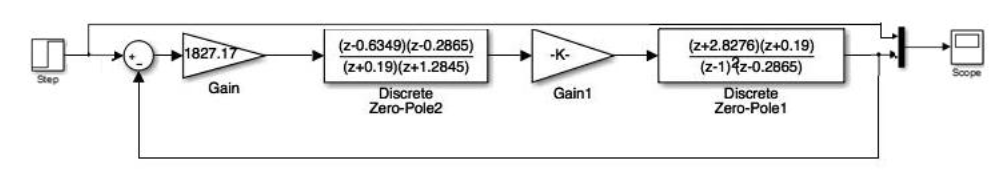
\includegraphics[width=1\linewidth]{images/diagrama2b.png}
            \caption{Diagrama do sistema.}
            \label{fig:diagram2b}
    \end{figure}

    \begin{figure}[H]
       \centering
            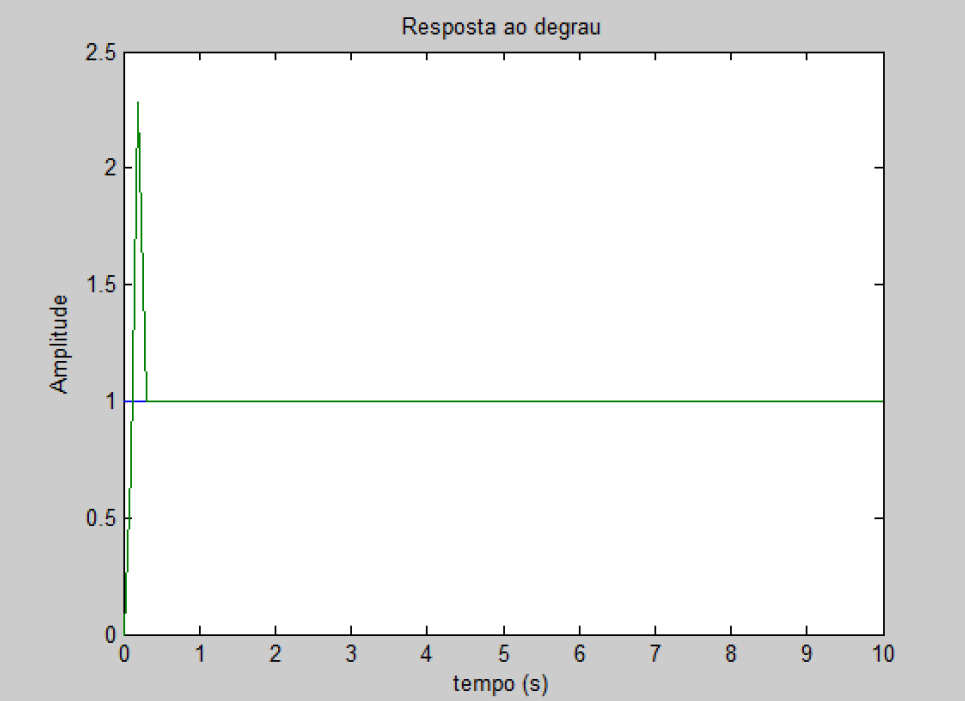
\includegraphics[width=.7\linewidth]{images/grafico2b.png}
            \caption{Resposta ao degrau.}
            \label{fig:graph2b}
    \end{figure}


    {\textbf{c)}}

    $$ p = max\{ 2,2 \} = 2 $$
    $$ n = 3-2 = 1 \implies k \geq n = 1 $$

    {Como k e p não sofrem alteração, o controlador permanece o mesmo, sendo}

    $$ G_{D}(z) = \frac{ 1827.17(z-0.6349)(z-0.2865) }{ (z+019)(z+1.2845) } $$


    {\textbf{d)}}

    \begin{figure}[H]
       \centering
            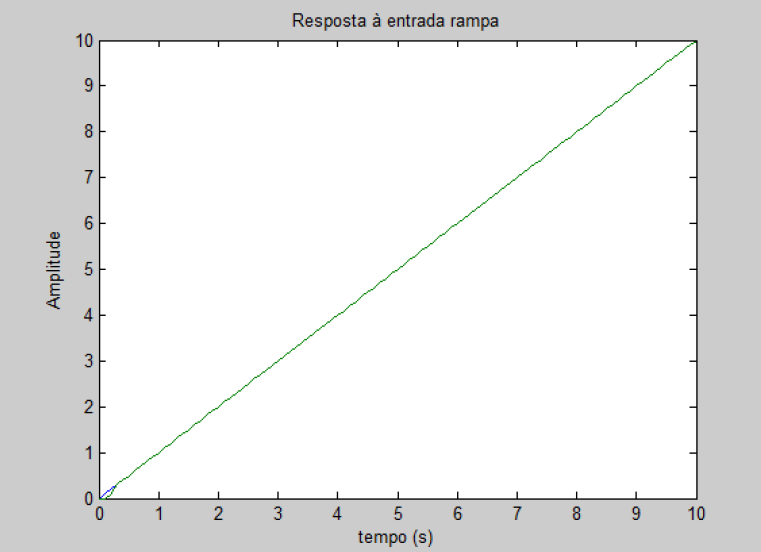
\includegraphics[width=.6\linewidth]{images/grafico2d.png}
            \caption{Resposta à rampa.}
            \label{fig:graph2d}
    \end{figure}


\section*{Questão 3}
    {\textbf{d)}}
    \begin{figure}[H]
       \centering
            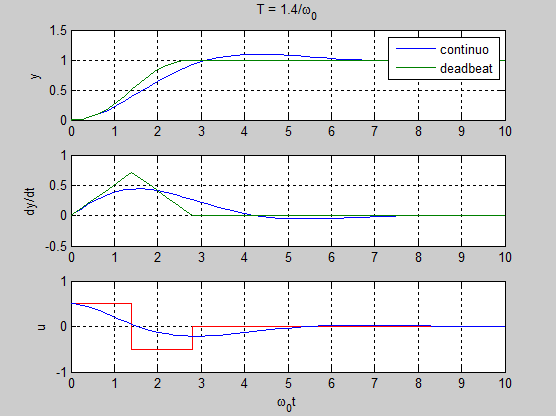
\includegraphics[width=.7\linewidth]{images/sim_t14s.png}
            \caption{Comparação das ações de controle para T = 1.4s.}
            \label{fig:sim1_4}
    \end{figure}
    \begin{figure}[H]
       \centering
            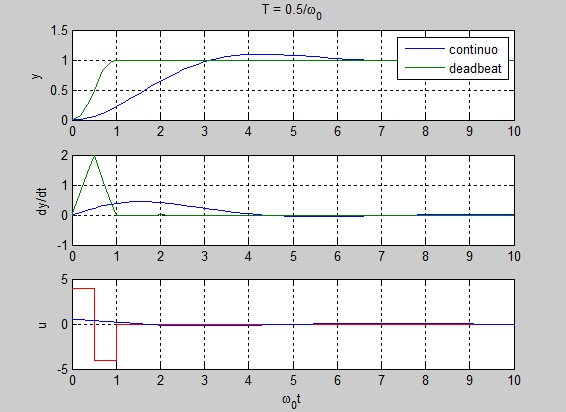
\includegraphics[width=.7\linewidth]{images/sim_t05s.png}
            \caption{Comparação das ações de controle para T = 0.5s.}
            \label{fig:sim0_5}
    \end{figure}
    \begin{figure}[H]
       \centering
            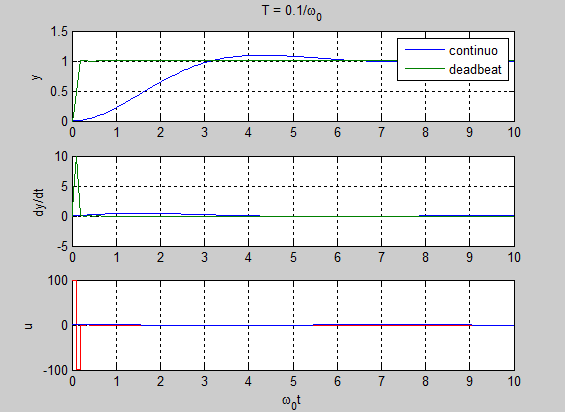
\includegraphics[width=.7\linewidth]{images/sim_t01s.png}
            \caption{Comparação das ações de controle para T = 0.1s.}
            \label{fig:sim0_1}
    \end{figure}

\end{document}
